%%%%%%%%%%%%%%%%%%%%%%%%%%%%%%%%%%%%%%%%%%%%%%%%%%%%%%%%%%%%%%%%%%%
%                                                                 %
%                            CHAPTER THREE                        %
%                                                                 %
%%%%%%%%%%%%%%%%%%%%%%%%%%%%%%%%%%%%%%%%%%%%%%%%%%%%%%%%%%%%%%%%%%%

\chapter{CAVITY-BASED CONFORMAL MESH ADAPTATION}
\label{chap:adapt}

\section{In Context}

The mesh adaptation methods in this work are both
conformal, general, and cavity-based.
They are conformal in the sense that the boundaries of all
elements (Section \ref{sec:def_complex}) are composed
of the set of entities expected by that element's
topological template (Section \ref{sec:topo_template}).
In other words, we avoid the ``hanging node" scenarios
introduced by non-conformal mesh modification techniques.
Typically, non-conformal mesh modification also restricts
itself to subdividing input elements into more elements,
or undoing such subdivisions which were done before.
Figure \ref{fig:hex_amr} illustrates such a method,
and clearly shows the hanging nodes introduced.

\begin{figure}
\begin{center}
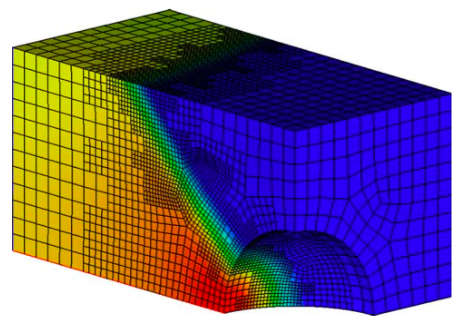
\includegraphics[width=0.6\textwidth]{hex_amr.png}
\caption{Non-conforming parent-child adaptive mesh refinement
\cite{kirk2006libmesh}}
\label{fig:hex_amr}
\end{center}
\end{figure}

Non-conforming meshes require additional support from
the PDE-solving code to deal with hanging nodes, and typically
no more than one level of refinement is allowed between adjacent
elements.
The more important limitation is due to non-conforming methods
typically being parent-child methods, which fundamentally limits
them to the topology of the coarse input mesh.
If this input mesh is more fine than necessary in some areas,
it cannot be coarsened.
If moving objects or object deformation cause input elements
to become highly compressed or even inverted, parent-child
refinement can never correct or prevent this.
For these reasons we take a general approach, employing
coarsening, swapping, and possibly other operations which are
able to coarsen beyond the input mesh and correct low-quality
elements in the input mesh.

We restrict ourselves to local cavity operations as well,
meaning that the transformation from input to output meshes
can be expressed as a series of cavity modifications, each
of which can in turn be expressed as a the removal of
a small number of mesh entities followed by the addition
of a small number of mesh entities.
In this case small means a number which can be bounded
by a constant and is not affected by the total number
of mesh entities.

The benefits of using local cavity operations are:
\begin{enumerate}
\item It allows more straightforward and reliable parallelization of
mesh adaptation (see Section \ref{sec:cavity_sched}).
\item It allows much more careful control of the effects that mesh
adaptation has on the simulation fields attached to the mesh.
\end{enumerate}

On the other hand, the set of known cavity operations
have been found by the trial and error of researchers,
and there are many properties which they are not guaranteed to
achieve.
The most successful set of cavity operators are those
which operate on simplex meshes, due ultimately to the
fact that a simplex is the simplest polytope of a given dimension,
and that more complex polytopes require exponentially more
complex considerations.
In our work, we separate cavity operators into three categories:
\begin{enumerate}
\item Refinement: create a strictly more detailed discretization
than the input. Guaranteed not to invert elements, but not to
preserve any element quality. Guaranteed to exactly preserve
the distribution of fields.
\item Coarsening: create a strictly less detailed discretization
than the input. No guarantees it can be done without reducing
or negating quality, so it must be checked.
By definition, cannot exactly preserve the distribution of the fields.
\item Shape correction: typically maintains similar level of detail,
modifies connectivity to improve minimum element quality.
There is no known method guaranteed to raise all elements to a quality
that is useful for simulation and adaptation, but heuristic
methods can achieve great results in practice \cite{klingner2008aggressive}.
\end{enumerate}

\section{Related Work}

There have been several iterations of the MeshAdapt
library developed at RPI.
One of the earliest publications by De Cougny and Shephard
\cite{de1999parallel} outlines the three basic steps and goes into some detail
on a use of independent sets for coarsening purposes
(an idea that we extend significantly in Section \ref{sec:indset}.
Later, much work was done by Li on anisotropy using the metric
tensor and the selection of operators for shape correction
\cite{li20053d,li2003mesh}.
Our implementations of tetrahedral edge swaps make use
of guidance on fast implementation by Olivier-Gooch \cite{freitag1997tetrahedral}.
Researchers at INRIA have provided useful mathematical foundations
for handling the anisotropic metric tensor field
\cite{frey2005,alauzet2006parallel,loseille2015parallel},
and work at the Catholic University of Louvain explored
the use of mesh adaptation to respond to moving objects
\cite{compere2010mesh}, a path we continue with our Omega\_h work.

\section{MeshAdapt Methods}
\label{sec:ma_methods}

The MeshAdapt library uses edge-based refinement templates for its refinement step.
The way these work is that all edges whose metric length exceeds some threshold
$l_{\text{up}} > 1$ are marked for refinement.
Then each element takes into account the subset of its edges which are marked
for refinement, and chooses one of many possible subdivision patterns
(refinement templates) based on this subset of edges.
Figure \ref{fig:tet_templates} illustrates these templates in the case of tetrahedra.
In fact, the center template shown for three marked edges has two variants which
are symmetric by reflection but not by rotation.
In total, this means there are 12 rotationally unique tetrahedron refinement templates.

\begin{figure}
\begin{center}
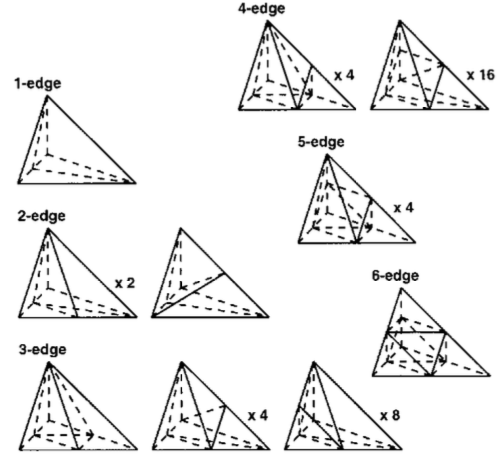
\includegraphics[width=0.6\textwidth]{tet_templates.png}
\caption{Tetrahedral refinement templates}
\label{fig:tet_templates}
\end{center}
\end{figure}

One benefit of the use of refinement templates is that adjacent elements can be refined
simultaneously, so all edges, faces, and regions of the mesh can be modified in
a nearly embarrassingly parallel fashion once the set of marked edges is identified.
Another benefit is that the gradation of the mesh is more explicitly controlled
compared to methods which split edges independently.
However, refinement templates have some drawbacks as well:
\begin{enumerate}
\item In some cases, a subset of the template is a polyhedron that cannot be
subdivided into tetrahedra without introducing an extra vertex within the
parent tetrahedron.
In particular, Sch{\"o}nhardt's polyhedron can appear (see Figure
\ref{fig:schonhardt}).
This reduces the predictability of refinement and makes it more difficult
to transfer solution.
\item Other cases introduce a geometric decision, such as the case
when all edges of a tetrahedron are refined, or even when two edges
of a triangle are refined. This also reduces predictability.
\item It takes substantial code to implement all rotationally unique
combinations for all the relevant element polytopes.
This increases the likelihood of errors and decreases the productivity
of modifying any aspect of refinement.
\item Due to the simultaneous nature of the operation and the difficulty
of predicting the outcome, it is prohibitively difficult to reject
a local portion of the refinement based on criteria such as new elements
being too low quality.
\end{enumerate}

\begin{figure}
\begin{center}
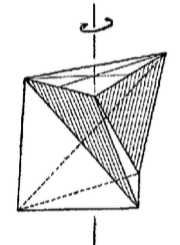
\includegraphics[width=0.25\textwidth]{schonhardt.png}
\caption{Sch{\"o}nhardt's irreducible polyhedron
\cite{Schonhardt1928}}
\label{fig:schonhardt}
\end{center}
\end{figure}

\section{Omega\_h Methods}
\label{sec:omega_h-adapt}

Focuses on serial aspects, i.e. single splits and
quality restrictions.

\section{Size Field Algorithms}
\label{sec:sf}

\subsection{Metric Storage and Interpolation}

Storage format is closely tied to interpolation scheme.
Describe:
\begin{enumerate}
\item MeshAdapt's way (eigendecomposed, rotation gets
linear plus gram-schmidt)
\item Omega\_h's way (linearization is the inverse,
as indicated by Alauzet), describe symmetric storage.
\item linear in square root, suggested as best by Alauzet.
Indicate expense of eigendecomposition.
\item linear in logarithm, suggested best by (cite Todd Michal)
and supported by (cite Alejandro Mota).
\end{enumerate}

Indicate last two may be better and are future work.

\subsection{Identity Size Field}

\subsection{Targeting an Element Count}

\section{Solution Transfer in a Cavity}

Emphasize numerical / performance advantage
over full-mesh methods.
Results can be included for each particular
method if it warrants one.

\subsection{Conserving Integral Quantities}

\section{Serial Adaptation Performance}

Both absolute performance and perhaps comparing
different methods.

%%% Local Variables:
%%% mode: latex
%%% TeX-master: t
%%% End:


